\documentclass[10pt,a4paper]{article}
\usepackage[utf8]{inputenc}
\usepackage{amsmath}
\usepackage{amsfonts}	%Gestion dans les environnements mathématiques.
\usepackage{amssymb}
\usepackage{bbm}		%Gestion des caractères pour les ensembles (N, Z, Q, R, C)
\usepackage{graphicx} 	%Gestion des images.
\usepackage{array}		%Gestion spécifique pour les tableaux.
						%Paramètres de placement dans les cellules: m, p, b. 
						%Avec dimensionnement de la colonne: m{2cm}.
\usepackage{multicol}	%Gère la mise en colonnes du texte.

\usepackage{fancyhdr}	%Gère la personnalisation des headers.
\usepackage{geometry}
\usepackage{marginnote}	%Gère la création de notes en marge du texte.
\usepackage{adjustbox}	%Options additionnelles de placement de l'image 
						%(left, right, center, outer and inner)
\usepackage{float}
\usepackage{rotating}	%Permet d'afficher une image, tournée de 90 degrés.
%-----------------------------------------------------------------------------
\title{Fourier, Laplace and Z transformations}
\author{Lucas Wälti}
\date{\today}
%-----------------------------------------------------------------------------
\pagestyle{fancy} 	%Types de headers standards: empty, plain (default),
					%							 headings, myheadings, fancy.
\fancyhf{}			%Clear le header et footer par défaut.
\rhead{Summary}
\lhead{Fourier, Laplace and Z transformations}	%Texte à droite, gauche et au centre du header.
\chead{}
\rfoot{}
\lfoot{}
\cfoot{Page \thepage}			%Texte du footer (ici: numéro de page).

\renewcommand{\headrulewidth}{0.5pt}
\renewcommand{\footrulewidth}{0pt}	%Lignes horizontales de séparation.
%-----------------------------------------------------------------------------
\begin{document}
\maketitle
\newpage
\tableofcontents
\thispagestyle{empty}	%Supprime le header et le footer pour cette page. 

\newpage
\section{Convolution Product}
For 2 functions $x(t)$ and $h(t)$ (usually denoting the impulse response of a LTI system), the \textbf{convolution product} is defined as: 
$$
y(t) = x(t) * h(t) = \int_{-\infty}^{\infty}{x(\tau)h(t-\tau)} d\tau
$$
\noindent
And in case of time discrete convolution:
$$
y[n] = x[n] * h[n] = \sum_{l=-\infty}^{\infty}{x[l]h[n-l]}
$$
\noindent
The product \textbf{commutes}, \textbf{associates} and \textbf{distributes}. 
By knowing the impulse response $h(t)$ of any LTI system, providing an input $x(t)$ to the system will produce an output $y(t) = x(t) * h(t)$. This can avoid solving a differential equation for this input. 

\section{Correlation}
For energy limited signals, given by the condition:
$$
\int_{-\infty}^{\infty}{\vert x(t)\vert ^2 dt} = E_x < \infty \text{, or for discret signals } \sum_{l=-\infty}^{\infty}{\vert x[l]\vert ^2} = E_x < \infty
$$
\noindent
The correlation is calculated as
$$
\varphi_{\mu \nu}(t) = \int_{-\infty}^{\infty}{x_\mu(\tau)x_\nu(t+\tau)} d\tau
$$
\noindent
If $\mu = \nu$, we speak of auto-correlation, while if $\mu \neq \nu$, we speak of the cross-correlation of the two signals. In case the signal is periodic, the integration happens on the interval of the signal, as follows:
$$
\tilde{\varphi}_{\mu \nu}(t) = \frac{1}{T_0}\int_{T_0}{x_\mu(\tau)x_\nu(t+\tau)} d\tau
$$
\noindent 
If the signals are discret, sum from 0 to N-1 and divide the sum by N. 

\section{Fourier Series}
Any periodic signal, limited and continuously differentiable in the interval of length $T_0$ can be written as a Fourier series: 
$$
\boxed{
\tilde{x}(t) = \sum_{k=-\infty}^{\infty}{c_ke^{j k \omega_0 t}}
} \text{ , } 
\omega_0 = \frac{2 \pi}{T_0}
$$
$$
\boxed{
c_k = \frac{1}{T_0} \int_{T_0}{\tilde{x}(t) e^{-j \omega_0 t} dt}
}
$$
\noindent
In case of real periodic signals $\tilde{x}(t)$, $\boxed{ c_{-k} = c_k^* }$
\subsection{Decomposition of the Fourier Series}
The coefficients $c_k$ can be rewritten as:
$$
c_k = 
\begin{cases} 
	\frac{a_k - jb_k}{2} & \text{ pour } k \in N \\
	a_0 				 & \text{ pour } k = 0
\end{cases}
\text{ avec } a_{-k} = a_k \text{ et } b_{-k} = b_k
$$
\noindent
Therefore the series can take the following form in the case of real periodic signals: 
$$
\boxed{
\tilde{x}(t) = a_0 + \sum_{k=1}^{\infty}{a_k \cos(k \omega_0 t)}
				   + \sum_{k=1}^{\infty}{b_k \sin(k \omega_0 t)}
}
$$
$$
a_0 = \frac{1}{T_0} \int_{T_0}{ \tilde{x}(t) dt } \text{ , }
a_k = \frac{2}{T_0} \int_{T_0}{ \tilde{x}(t) \cos(k \omega_0 t) dt } \text{ , }
b_k = \frac{2}{T_0} \int_{T_0}{ \tilde{x}(t) \sin(k \omega_0 t) dt }
$$

It is important to see that for even functions $\tilde{x}(t)$ all $b_k = 0, \forall k \geq 1$, while for uneven functions, all $a_k = 0, \forall k \geq 0$. 

\subsection{Parseval Theorem of the Fourier Series}
$$
\boxed{
\frac{1}{T_0} \int_{T_0}{\vert \tilde{x}(t) \vert^2 dt}
= \sum_{k=-\infty}^{\infty}{ \vert c_k \vert^2 }
= \vert c_0 \vert^2 + 2 \sum_{k=1}^{\infty}{ \vert c_k \vert^2 }
}
$$
\noindent
This result can be proved as follows: 
$$
\tilde{x}(t) = \sum_{k=-\infty}^{\infty}{c_k e^{j k \omega_0 t}}
$$
$$
\tilde{x}^*(t) = \sum_{k'=-\infty}^{\infty}{c_{k'}^* e^{-j k' \omega_0 t}}
$$
$$
P = \frac{1}{T_0} \int_{T_0}\vert \tilde{x}(t) \vert^2 dt
  = \frac{1}{T_0} \int_{T_0} \tilde{x}(t) \tilde{x}^*(t) dt
  = \frac{1}{T_0} \sum_{k=-\infty}^{\infty} \sum_{k'=-\infty}^{\infty} 
    \underbrace{c_k c_{k'}^*}_{= \vert c_k^2 \vert}
    \underbrace{\int_{T_0} e^{j (k-k') \omega_0 t} dt}_{T_0 \cdot \delta(k-k')}
$$
As $k = k'$ because of the Dirac function $\delta(k-k')$ that is equal to $0$ if $k \neq k'$. We then find that: 
$$
P = \sum_{k=-\infty}^{\infty}{ \vert c_k \vert^2 } \qquad \square
$$
The result of the integral ($\int_{T_0} e^{j (k-k') \omega_0 t} dt$) will be discussed later on, when working on the Fourier transformation. 

\subsection{Time Shift of the Fourier Signal}
A time shift of the signal will result in a phase shift of the coefficient $c_k$ of the series. 
$$
\tilde{x}(t - \tau) = \sum_{k=-\infty}^{\infty} {c_ke^{j k \omega_0 (t - \tau)}}
					= \sum_{k=-\infty}^{\infty} {c_ke^{-j k \omega_0 \tau} e^{j k \omega_0 t}}
					= \sum_{k=-\infty}^{\infty} {c_k(\tau) e^{j k \omega_0 t}}
$$
Hence the phase shift is equal to $-k \omega_0 \tau$. 

\subsection{Periodic Convolution}
For two periodic signals $\tilde{x}_1(t)$ and $\tilde{x}_2(t)$, we define on a period length (because of convergence issues) the \textit{periodic convolution}:
$$
\tilde{y}(t) = \tilde{x}_1(t) * \tilde{x}_2(t) 
			 = \int_{T_0}{\tilde{x}_1(\tau) \tilde{x}_2(t-\tau)} d\tau
$$ 
The the coefficients of the Fourier series follow the rule: 
$$
\boxed{ c_{yk} = T_0 \cdot c_{1k} \cdot c_{2k} }
$$


\section{The Fourier Transformation FT}
The advantage of the Fourier transformation is to enable us to transform not periodical signals. The Fourier series can only work for periodic signals! Note here that both transformations can be multiplied by a factor $\frac{1}{\sqrt{2\pi}}$, depending on the convention. 
$$
\boxed{
X(\omega) = \int_{-\infty}^{\infty} x(t) e^{-j \omega t} dt
}
$$
$$
\boxed{
x(t) = \frac{1}{2\pi} \int_{-\infty}^{\infty} X(\omega) e^{j \omega t} d\omega
}
$$
The condition for the existence of the transformation is that $x(t)$ is differentiable on a finite number of places and that it is absolutely integrable:
$$
\int_{-\infty}^{\infty} \vert x(t) \vert dt < \infty
$$

\subsection{Parseval Theorem for the Fourier Transformation}
$$
\boxed{
E_x = \int_{-\infty}^{\infty} \vert x(t) \vert ^2 dt 
	= \frac{1}{2\pi} \int_{-\infty}^{\infty} \vert X(\omega) \vert^2 d\omega
}
$$
Of course this does not converge for periodic signals. The Parseval Theorem for the Fourier series has to be used instead in case of periodic signals. For the sake of generality, the theorem is given for two signals: 
$$
E_{\mu \nu} = \int_{-\infty}^{\infty} x_\mu^*(t)x_\nu(t) dt 
			= \frac{1}{2\pi}\int_{-\infty}^{\infty} X_\mu^*(\omega)X_\nu(\omega) d\omega
$$
\subsection{Example of the Fourier Transformation}
Let us prove the following result: 
$$
\boxed{
\frac{1}{2\pi} \int_{-\infty}^{\infty} e^{j\omega_0t} dt = \delta(\omega_0)
}
$$
Let us set $x(t) = \delta(t-t')$:
$$
X(\omega) = \int_{-\infty}^{\infty} x(t) e^{-j \omega t} dt
		  = \int_{-\infty}^{\infty} \delta(t-t') e^{-j \omega t} dt
\qquad \text{ with } \qquad \delta(t-t') e^{-j \omega t} \neq 0 \text{ for } t = t'
$$
which yields,
$$
X(\omega) = e^{-j \omega t'}, \qquad x(t) = \delta(t-t')
$$
By applying the inverse transform,
$$
x(t) = \delta(t-t') 
	 = \frac{1}{2\pi} \int_{-\infty}^{\infty} X(\omega) e^{j \omega t} d\omega
	 = \frac{1}{2\pi} \int_{-\infty}^{\infty} e^{j \omega (t-t')} d\omega
$$
which proves
$$
\delta(t-t') = \frac{1}{2\pi} \int_{-\infty}^{\infty} e^{j \omega (t-t')} d\omega
\qquad \square
$$

\subsection{Relation between the transformation and the series}
From the relations we saw until now: 
$$
\tilde{x}(t) = \sum_{k=-\infty}^{\infty}{c_ke^{j k \omega_0 t}}
\qquad
c_k = \frac{1}{T_0} \int_{T_0}{\tilde{x}(t) e^{-j \omega_0 t} dt}
$$
and
$$
x(t) = \frac{1}{2\pi} \int_{-\infty}^{\infty} X(\omega) e^{j \omega t} d\omega
\qquad
X(\omega) = \int_{-\infty}^{\infty} x(t) e^{-j \omega t} dt
$$
it comes that
$$
\boxed{
c_k = \frac{1}{T_0} X(k \omega_0) \qquad \Leftrightarrow \qquad T_0 c_k = X(k \omega_0)
}
$$
This means that $X(\omega)$ envelops the coefficients $c_k$ with a factor $T_0$. The $c_k$ are separated by a distance $\omega_0 = \frac{2\pi}{T_0}$.

\subsection{Linear Differential Equations with constant coefficients}
A differential equation of order N has the form: 
$$
\sum_{l=0}^{N} a_l \frac{d^l}{dt^l}y(t) = \sum_{m=0}^{M} b_m \frac{d^m}{dt^m}x(t) 
$$
And by knowing that:
$$
\frac{d^n}{dt^n}x(t) \quad \longleftrightarrow \quad (j\omega)^nX(\omega)
$$
The equation can be written after transformation as:
$$
Y(\omega)\sum_{l=0}^{N}(j\omega)^l a_l = X(\omega)\sum_{m=0}^{M}(j\omega)^m b_m
$$
Hence the \textbf{transfer function} $H(\omega)$: 
$$
\boxed{
H(\omega) = \frac{Y(\omega)}{X(\omega)}
		  = \frac{\sum_{m=0}^{M}(j\omega)^m b_m}
		         {\sum_{l=0}^{N}(j\omega)^l a_l}
}
$$
The phase and magnitude of the transfer function are usually represented in logarithmic scales, typically with a \textit{Bode-Diagram}. 

\section{The Time Discrete Fourier Transformation TDFT}
Time is now discrete so the normalisations are necessary, with the sampling period $T_s$: 
$$
n = \frac{t}{T_s}
$$
$$
\Omega = \omega T_s = 2\pi f \cdot \frac{1}{f_s}
$$
This is due to the fact that $ \phi(t) = e^{j \omega t} = e^{j \omega nT_s} = e^{j \Omega n} $.
The transformations are then given as follows: 
$$
\boxed{
X(\Omega) = \sum_{n=-\infty}^{\infty} x[n] e^{-j \Omega n}
}
$$
$$
\boxed{
x[n] = \frac{1}{2\pi} \int_{2\pi} X(\Omega)e^{j \Omega n} d\Omega
}
$$
In order for the transformation to exist, the sequence has to be \textit{stable}, hence:
$$
\vert X(\Omega) \vert = \sum_{n=-\infty}^{\infty} \vert x[n] \vert < \infty, \quad \forall \; \Omega
$$
It is important to see that the spectrum is \textbf{periodical}. It can be expressed as:
$$
\boxed{
X(\Omega) = X(\Omega + 2\pi), \quad \forall \; \Omega
}
$$

\subsection{Infinite Sum of Complex Exponentials}
With the following series in mind, with $\vert a \vert < 1$: 
$$
\sum_{k=0}^{N} a^k = \frac{1 - a^{N+1}}{1 - a}
\quad \longleftrightarrow \quad 
\sum_{k=0}^{\infty} (ae^{x})^k = \frac{1}{1 - ae^x}
$$
We have:
$$
\sum_{k=-\infty}^{\infty} (ae^{jx})^k = \sum_{k=0}^{\infty} (ae^{jx})^k + 
										\sum_{k=0}^{\infty} (ae^{-jx})^k 
									   	\underbrace{-(ae^{jx})^0}_{\text{*)}}
$$
$$
 = \frac{1}{1-ae^{jx}} + \frac{1}{1-ae^{-jx}} - 1 
 = \frac{2 - a(e^{jx}+e^{-jx})}{1 - a(e^{jx}+e^{-jx}) + a^2} - 1
 \underbrace{=}_{\lim_{a \to 1}} 1 - 1 = 0
$$
*) If not subtracted here, it would be present two times in the sums otherwise. 

If we take the definition of the series with $a = 1$ and let $e^x = e^{\pm j 2 \pi n} = 1$, then the series diverges towards infinity. For any other value of $e^x$, the series is equal to zero. This is equivalent to a series of Dirac impulses!

As a final result, by letting $a=1$ and $x=\Omega$ in the previous equations:
$$
\boxed{
\sum_{n=-\infty}^{\infty} e^{-j \Omega n} = 2\pi \sum_{r=-\infty}^{\infty} \delta(\Omega - 2\pi r)
}
$$
This result may come handy when calculating a TDFT. 


\subsection{Parseval Theorem for the TDFT}
The \textit{Energy Signal} is given as: 
$$
E_x = \sum_{n=-\infty}^{\infty} \vert x[n] \vert^2 = \frac{1}{2\pi} \int_{2\pi} \vert X(\Omega) \vert^2 d\Omega
$$
$\vert X(\Omega) \vert^2$ describes the Spectrum of the Energie Density. The Energy Signal of two overlapping signals is given as: 
$$
E_{xy} = \sum_{n=-\infty}^{\infty} x[n]y^*[n] = \frac{1}{2\pi} \int_{2\pi} X(\Omega)Y^*(\Omega) d\Omega
$$

\subsection{Transfer Function for LTI System}
$$
y[n] = x[n]*h[n] = \sum_{l=-\infty}^{\infty}{x[l]h[n-l]}
				 = \sum_{l=-\infty}^{\infty}{h[l]x[n-l]}
$$
Therefore, we can express the transfer function as:
$$
Y(\Omega) = H(\Omega)X(\Omega) \leftrightarrow 
\boxed{H(\Omega) = \frac{Y(\Omega)}{x(\Omega)}}
$$
With the \textbf{stability} condition:
$$
\boxed{ \sum_{n=-\infty}^{\infty} \vert h[n]\vert < \infty }
$$

\subsection{Linear Differential Equations with constant coefficients}
A differential equation is given as:
$$
\sum_{l=0}^{N} a_l y[n-l] = \sum_{m=0}^{M} b_m x[n-m]
$$
After transformation:
$$
Y(\Omega) \sum_{l=0}^{N} a_l e^{-j \Omega l} = 
X(\Omega) \sum_{m=0}^{M} b_m e^{-j \Omega m}
$$
Hence
$$
H(\Omega) = \frac{Y(\Omega)}{X(\Omega)} = \frac{\sum_{m=0}^{M} b_m e^{-j \Omega m}}{\sum_{l=0}^{N} a_l e^{-j \Omega l}}
$$

\begin{list}{-}{}
\item \textit{First Order}: The denominator only has values for $l = 0,1$.
\item \textit{Second Order}: The denominator only has values for $l = 0,1,2$.
\item \textit{Higher Order}: They can be built from First and Second order systems. 
\end{list}


\section{Signal Sampling and Reconstruction}
A time continuous signal $x(t)$ is modulated by a sampling function $s(t)$ at a rate $\omega_s$. 
$$
s(t) = \sum_{n=-\infty}^{\infty} \delta(t-nT_s) \quad \leftrightarrow \quad 
S(\omega) = \frac{2\pi}{T_s} \sum_{r=-\infty}^{\infty} \delta(\omega - r \omega_s)
$$
Therefore we have the sampled signal $x_s(t)$:
$$
x_s(t) = x(t)s(t) = \sum_{n=-\infty}^{\infty} x(nT_s)\delta(t - nT_s)
$$
$$
\boxed{
X_s(\omega) = \frac{1}{2\pi} X(\omega)*S(\omega)
			= \frac{1}{T_s} \sum_{r=-\infty}^{\infty} X(\omega - r\omega_s)}
$$
Which proves, the spectrum of a time discrete signal is \textbf{periodical}! 

\subsection{The Shannon Sampling Theorem}
With $\omega_s$ the sampling rate and $\omega_g$ the maximal rate of the signal:
$$
\boxed{
\omega_s \geq 2\omega_g \longleftrightarrow T_s \leq \frac{\pi}{\omega_g}
}
$$
This means that $X(\omega) = 0$ for $\vert\omega\vert > \omega_g$. This means the width of the Spectrum has to be equal or smaller than the sampling rate. Otherwise, there is some overlapping and information is lost. 

\subsection{Signal Reconstruction}
By applying a low pass to the signal given as $$H_r(\omega) = T_s$$ for $\vert \omega \vert \leq \omega_r$. A common choice for $\omega_r$ is $\frac{\pi}{T_s}$.
$$
h_r(t) = \frac{1}{2\pi} \int_{-\infty}^{\infty} H_r(\omega)e^{j\omega t} d\omega
	   = \frac{1}{2\pi} \int_{-\omega_r}^{\omega_r} T_se^{j\omega t} d\omega
	   = \frac{1}{2\pi} \int_{-\frac{\pi}{T_s}}^{\frac{\pi}{T_s}} T_se^{j\omega t} d\omega
	   = \frac{T_s}{\pi t} \sin(\omega_r t)
	   = \text{si}(\frac{\pi t}{T_s})
$$
Hence
$$
x_r(t) = \int_{-\infty}^{\infty} x_s(\tau) h_r(t-\tau)d\tau
	   = \sum_{n=-\infty}^{\infty} \int_{-\infty}^{\infty} x(nT_s) \delta(\tau-nT_s)h_r(t-\tau) d\tau
	   = \sum_{n=-\infty}^{\infty} x(nT_s) h_r(t-nT_s)
$$
$$
\boxed{
x_r(t) = \frac{\omega_rT_s}{\pi} \sum_{n=-\infty}^{\infty} x(nT_s) \text{si}(\omega_r(t-nT_s))
}
$$
The Reconstruction of a sampled signal is done by the summation of a multitude of si-functions!

\subsection{Sampling in Frequency Domain}
The function 
$$
P(\omega) = \sum_{n=-\infty}^{\infty} \delta(\omega-k\omega_p) \quad
\leftrightarrow \quad
p(t) = \frac{T_p}{2\pi} \sum_{r=-\infty}^{\infty} \delta(t-rT_p)
$$
is used for the sampling of the signal. The signal in time domain of a sampled spectrum is \textbf{periodical} with a period $T_p$:
$$
x_p(t) = x(t) * p(t) = \frac{T_p}{2\pi} \sum_{r=-\infty}^{\infty} x(t - rT_p)
$$
\subsubsection{Sampling Theorem in Frequency Domain}
To avoid an overlap of the time-signals:
$$
\boxed{ T_p \geq 2T_g }
$$
as the time-periodical signal is $2T_g$ wide, $T_p$ must guaranty that each chunk of signal has enough room to avoid overlapping. 

\section{The Laplace Transformation LT}
The Laplace transformation allows some better convergence properties than the Fourier transform. By setting:
$$
s = \sigma + j\omega 
$$
The Laplace transform is given as:
$$
\boxed{
X(s) = \int_{-\infty}^{\infty} x(t)e^{-st}dt}
$$
$$
\boxed{
x(t) = \frac{1}{2\pi j} \int_{\sigma-j\infty}^{\sigma+j\infty} X(s)e^{st}ds
	 = \frac{1}{2\pi} \int_{-\infty}^{\infty} X(\sigma + j\omega)e^{(\sigma + j\omega)t}d\omega}
\quad \textbf{\footnotemark}
$$
\footnotetext{
The presence of $j$ here is due to the change of variables from the FT:
$s = \sigma + j\omega$ which with partial derivation gives $ds = jd\omega \longrightarrow d\omega = \frac{ds}{j}$
}

Note: To solve the inverse transform, one can use the \emph{Residue Theorem} as follows:
$$
\frac{1}{2\pi j}\oint_C X(s)e^{st}ds = \sum_{k=1}^K Res\{X(s),s_k\}
$$


Considering that
$$
X(s) = X(\sigma+j\omega) = \int_{-\infty}^{\infty} (x(t)e^{-\sigma t})e^{-j\omega t}dt
$$
the LT can be interpreted as a FT:
$$
L(x(t)) = F(x(t)e^{-\sigma t})
$$
\begin{list}{•}{}
\item $\sigma > 0$: damping
\item $\sigma < 0$: amplification
\end{list}
In order for the LT to exist and to \textbf{converge}, with $\sigma_0$ providing the limit for the convergence domain: 
$$
\int_{-\infty}^{\infty} \vert x(t) \vert e^{-\sigma_0t} < \infty
$$
\textbf{IMPORTANT}: If the \emph{Imaginary Axis} $ \in \textit{Convergence Domain}$ then the FT converges also!

\subsection{The Unilateral Laplace Transformation}
This is useful to study the response of systems to a stimulation.
$$
X_+(s) = \int_{0}^{\infty} x(t)e^{-st}dt
$$
$$
x(t) = \frac{1}{2\pi j} \int_{\sigma-\infty}^{\sigma+\infty} X_+(s)e^{st}ds
$$
\subsection{Linear Differential Equations using the LT}
From the differential equation:
$$
\sum_{l=0}^{N} a_l \frac{d^l}{dt^l}y(t) = \sum_{m=0}^{M} b_m \frac{d^m}{dt^m}x(t) 
$$
The transfer function of the system can be expressed as:
$$
\boxed{
H(s) = \frac{Y(s)}{X(s)} = \frac{\sum_{m=0}^{M} b_m s^m}{\sum_{l=0}^{N} a_l s^l}
}
$$

\subsection{Convergence of the Laplace Transformation}
From the condition for the convergence, which provides a value for $\sigma_0$:
$$
\int_{-\infty}^{\infty} \vert x(t) \vert e^{-\sigma_0t} < \infty
$$
The Convergence Domain (CD) has following properties:
\begin{enumerate}
\item The CD is parallel to the imaginary axis in the s-plane.
\item If the Laplace Transform is rational, then there is no Pole within the CD.
\item If $x(t)$ is \textbf{finite in time}, and there is at least one value of $s$ that lets the LT converge, then the whole s-plane is a CD.
\item If $x(t)$ is a \textbf{right hand signal}, then all values of s with $Re(s) > \sigma_0$ are in the CD too. 
\item If $x(t)$ is a \textbf{left hand signal}, then all values of s with $Re(s) < \sigma_0$ are in the CD too. 
\item If $x(t)$ is \textbf{infinite in time}, then points 4 and 5 apply at the same time. 
\end{enumerate}

\newpage
\section{The z-Transformation ZT}
This transformation is a generalisation of the TDFT. It offers a stronger convergence, is usually simpler to handle with analytic problems and the complex writing is introduced by time discrete signals.
The bilateral ZT is given as:
$$
z = re^{j\omega}
$$
$$
\boxed{
X(z) = \sum_{n=-\infty}^{\infty} x[n] z^{-n}
}
$$
$$
\boxed{
x[n] = \frac{1}{2\pi j} \oint_C X(z)z^{n-1} dz
}
$$
$C$: Integration way along a closed circuit anti-clockwise within the convergence domain.
$X(z)$ can also be unilateral: 
$$
X_+(z) = \sum_{n=0}^{\infty} x[n] z^{-n}
$$

\subsection{Convergence of the z-Transformation}
The condition for the convergence is:
$$
\sum_{n=-\infty}^{\infty} \vert x[n]r^{-n} \vert < \infty
$$
The convergence properties come from the properties of the Laurent series. 
\begin{enumerate}
\item The Convergence Domain (CD) is \textbf{a ring or a disc around the origin} of the z-plane!

$0 \leq R_1 < \vert z \vert < R_2 \leq \infty$
\item The TDFT converges only if the CD of the z-Transform contains the unit circle. 
\item The CD contains no Pole.
\item If $x[n]$ is a sequence of finite length, then the whole z-plane is a CD. Excepted maybe for $z = 0$ and/or $\vert z \vert = \infty$.
\item If $x[n]$ is a right hand signal, the CD is the outer part of the circle containing the furthest Pole. 
\item If $x[n]$ is a left hand signal, the CD is the inner part of the circle containing the closest Pole. 
\item If $x[n]$ has no limit for $n$ (left and right), the CD is a ring free of any Pole, containing the circle $\vert z \vert = r_0$.
\item The CD is a one piece domain and has no detached sections. 
\end{enumerate}

\subsection{Comparison to the TDFT}
For $z = e^{j\Omega}$ with $\vert z \vert = 1$, the z-transformation becomes:
$$
\text{(ZT)} \quad
X(z) = \sum_{n=-\infty}^{\infty} x[n] z^{-n}
	 = \sum_{n=-\infty}^{\infty} x[n] (e^{j\Omega})^{-n} 
	 = \sum_{n=-\infty}^{\infty} x[n] e^{-j\Omega n} 
	 = X(\Omega) \quad \text{(TDFT)}
$$
For $z = re^{j\Omega}$ with $\vert z \vert = r$, the ZT can expressed as a TDFT:
$$
X(z) = X(re^{j\Omega}) = \sum_{n=-\infty}^{\infty} (x[n]r^{-n}) e^{-j\Omega n}
$$
As said above, the TDFT converges only if the CD of the z-Transform contains the unit circle.

\subsection{Residue Theorem}
The computation of the inverse ZT being given as:
$$
x[n] = \frac{1}{2\pi j} \oint_C X(z)z^{n-1} dz
$$
The complex integral on a closed path can be computed using the \textbf{Residue Theorem}:
$$
\boxed{
\oint_C f(z)dz = 2\pi j \sum_{k=1}^K Res\{f(z),z_k\}
}
$$
with $K$ the number of poles contained in the integration path $C$. For each pole $z_k$, the residue is calculated as:
$$
f(z) = \frac{A(z)}{(z-z_k)^m}
$$
$$
\boxed{
Res\{f(z),z_k\} = \frac{1}{(m-1)!} \frac{d^{m-1}}{dz^{m-1}} A(z) \vert_{z = z_k}
}
$$
with $k \in [1,K]$.

In our case $f(z) = X(z)\cdot z^{n-1}$.

To calculate Integrals of the form:
$$
\int_{-\infty}^{\infty} f(x) e^{i\omega x} dx = \int_{-\infty}^{\infty} \frac{p(x)}{q(x)} e^{i\omega x} dx
$$
with 
$ f(x) = \frac{p(x)}{q(x)} $ where $q$ and $p$ are \emph{polynomial} functions so that $ q(x) \neq 0, \forall x \in R $ and $\text{deg}(q) - \text{deg}(p) \geq 2 $. Then only the residues in the upper part of the complex plane must be included when solving the integral. 
If the exponential is negative or for negative values of $\omega$ ($\omega \leq 0$), only the poles of the lower part of the complex plain must be included. 

\subsection{Transition from the LT to the ZT}
There are many ways of numerically representing a function. Depending on how a function is represented, the relation between the LT and ZT will change. This transition is important for the implementation of filters, controllers, etc... that where derived in the Laplace domain and that need to be numerically implemented. 

\subsubsection{Integral Substitution}
An integration from $0$ to $t_k$ is given by:
$$
y(t_k) = \underbrace{\int_{0}^{t_{k-1}} x(t) \: dt}_{=y_{k-1}} + \underbrace{\int_{t_{k-1}}^{t_{k}} x(t) \: dt}_{= \Delta y_k}
$$
\paragraph{Rectangle Approximation}
We express $\Delta y_k$ as 
$$
\Delta y_k = x_k h
$$
Therefore $$ y_k = y_{k-1} + x_k h $$
$$ Y(z) = Y(z)z^{-1} + X(z)h $$
hence
$$
\frac{Y(z)}{X(z)} = \frac{h}{1-z^{-1}} = \frac{hz}{z-1} \quad \equiv \quad \frac{1}{s} = \frac{Y(s)}{X(s)}
$$
Which means we can substitute $s$ by
$$
\boxed{
s \: \hat{=} \: \frac{z-1}{hz}
}
$$

\paragraph{Trapeze Approximation}
Also called \emph{Tustin} or \emph{Bilinear Transform}. We express this time $\Delta y_k$ as 
$$
\Delta y_k = \frac{h}{2}(x_{k-1} + x_k)
$$
Therefore
$$
y_k = y_{k-1} + \frac{h}{2}(x_{k-1} + x_k)
$$
$$
Y(z) = Y(z)z^{-1} + \frac{h}{2}(X(z)z^{-1} + X(z))
$$
hence
$$
\frac{Y(z)}{X(z)} = \frac{h}{2} \frac{z+1}{z-1} \quad \equiv \quad \frac{1}{s} = \frac{Y(s)}{X(s)}
$$
Which means we can substitute $s$ by
$$
\boxed{
s \: \hat{=} \: \frac{2}{h} \frac{z-1}{z+1} \quad \Leftrightarrow \quad 
z \: \hat{=} \: \frac{1 + \frac{h}{2}s}{1 - \frac{h}{2}s} 
}
$$
\subsection{Pre-warping of the Bilinear Transform}
With the previous result:
$$
s \: \hat{=} \: \frac{2}{h} \frac{z-1}{z+1} \quad \Leftrightarrow \quad 
z \: \hat{=} \: \frac{1 + \frac{h}{2}s}{1 - \frac{h}{2}s} 
$$
the behaviour of the digital transfer function will differ from the continuous one when the frequency reaches the Nyquist frequency. This is due to the warping of the s-domain into the z-domain. 

Considering the frequency only, we can write:
$$
z = e^{j\omega_d T} = \frac{1+j\frac{\omega_a}{2} T}{1-j\frac{\omega_a}{2} T}
$$
which shows that $\omega_a \neq \omega_d$ (approx. linear for low frequencies):
$$
\omega_d = \frac{1}{jT} \text{ln}\left(\frac{1+j\frac{\omega_a}{2} T}{1-j\frac{\omega_a}{2} T}\right)
$$

Therefore the frequency warping can be expressed as follows:
\begin{align*}
H_d(z) = H_d(e^{j\omega_d T}) 
	  &= H_a\left(\frac{2}{T} \frac{e^{j\omega_d T}-1}{e^{j\omega_d T}+1}\right) \\
	  &= H_a\left(\frac{2}{T} \cdot \frac{e^{j\omega_d T/2}(e^{j\omega_d T/2}-e^{-j\omega_d T/2})}
	  									 {e^{j\omega_d T/2}(e^{j\omega_d T/2}+e^{-j\omega_d T/2)}}\right) \\
	  &= H_a\left(j\frac{2}{T} \cdot \frac{\sin(\omega_d T/2)}{\cos(\omega_d T/2)}\right) \\
	  &= H_a\left(j\frac{2}{T} \cdot \tan(\omega_d T/2)\right)
\end{align*}
This shows that every point on the unit circle in the discrete-time filter z-plane, $z=e^{j\omega T}$ is mapped to a point on the $j\omega$ axis of the s-plane, $s=j\omega_a$. Hence the discrete-time to continuous-time frequency mapping of the bilinear transform:
$$
\boxed{
\omega_a = \frac{2}{T} \tan\left( \omega_d \frac{T}{2} \right) \quad \Leftrightarrow \quad
\omega_b = \frac{2}{T} \tan^{-1}\left( \omega_a \frac{T}{2} \right)
}
$$
This means the \emph{discrete-time filter} behaves at frequency $\omega_d$ the same way the \emph{continuous-time filter} behaves at frequency $\omega_a = \frac{2}{T} \tan\left( \omega_d \frac{T}{2} \right)$. 

Finally, given a specific frequency $\omega_0$, we can pre-warp this frequency when applying the Bilinear Transform as follows: 
$$
\boxed{
s \: \hat{=} \: \frac{\omega_0}{\tan\left(\frac{\omega_0 T}{2}\right)} \frac{z-1}{z+1} 
}
$$

Note that for $\omega_0 \rightarrow 0$, $s \: \hat{=} \: \frac{2}{h} \frac{z-1}{z+1}$. 

\subsection{Matched Z-transform method}
Also called \emph{Zero-Pole Matching Method} is a pretty straight forward method. It is applicable with a few steps:
\begin{enumerate}
\item Map the poles and zeros of the s-plane to the z-plane with the transformation $z = e^{sT}$. This provides the corresponding new transfer function in the z-domain. 
\item Add zeros at infinity, which corresponds to multiplying the previously obtained transfer function by $(z+1)^n$ in order to have the same degree between the numerator and denominator of the transfer function. 
\item Retrieve zeros to make the function strictly proper (deg(numerator)$<$deg(denominator)). 
\item Calculate the DC-gain of both discrete-time and continuous time transfer functions and multiply the discrete-time transfer function by a gain $k_d$ such as $\text{DC-gain}(G(s)) = \text{DC-gain}(G(z)) \cdot k_d$.
\end{enumerate}

The DC-gain is obtained by setting $s = 0$ and $z = 1$ respectively. 

\subsection{ZOH Approach (Zero Order Hold)}
To apply a discrete signal to a continuous plant, a DA conversion is required. The most commonly used approach is the \emph{Zero Order Hold} method, where a discrete value will be hold until a second command value is emitted. This signal form will affect the discrete system and has to be accounted for. The signal sequence $v[k]$ goes through following blocks, until the output $Y(s)$: 
$$
v[k] \longrightarrow \text{ZOH} \longrightarrow G(s) \longrightarrow Y(s) \longrightarrow \text{AD} \longrightarrow y[k]
$$ 
We can express the ZOH as a series of steps, as the discrete values are hold:
$$
\text{ZOH} = v(t) = \sum_{k=0}^{\infty} v[k]_{\text{hold}} = \sum_{k=0}^{\infty} v[k]\Big( u(t-kT)-u(t-(k+1)T) \Big) 
$$
Hence
$$
V(s) = \sum_{k=0}^{\infty} v[k] \Big(\frac{1}{s}e^{-kTs} - \frac{1}{s}e^{-(k+1)Ts} \Big)
	 = \frac{1 - e^{-Ts}}{s} \sum_{k=0}^{\infty} v[k]e^{-kTs}
$$
Therefore
\begin{align*}
Y(s) &=  V(s) \cdot G(s) \\
  	 &= \frac{1 - e^{-Ts}}{s} \sum_{k=0}^{\infty} v[k]e^{-kTs} \cdot G(s) \\
  	 z = e^{sT} &\Rightarrow \frac{1 - z^{-1}}{s} \sum_{k=0}^{\infty} v[k]z^{-k} \cdot G(s) \\
Y(s) &= (1 - z^{-1})\frac{G(s)}{s} V(z)
\end{align*}
Finally
$$
\boxed{
H(z) = \frac{Y(z)}{V(z)} = (1-z^{-1})\cdot \mathcal{Z} \Big( \mathcal{L}^{-1}\Big( \frac{G(s)}{s} \Big) \Big)_{t = kT}
}
$$

\newpage
\section{Lists of Properties}
\subsection{Continuous Fourier transformation}
$$
X(\omega) = \int_{-\infty}^{\infty} x(t) e^{-j \omega t} dt \qquad
x(t) = \frac{1}{2\pi} \int_{-\infty}^{\infty} X(\omega) e^{j \omega t} d\omega
$$
\begin{figure}[H]
\centering
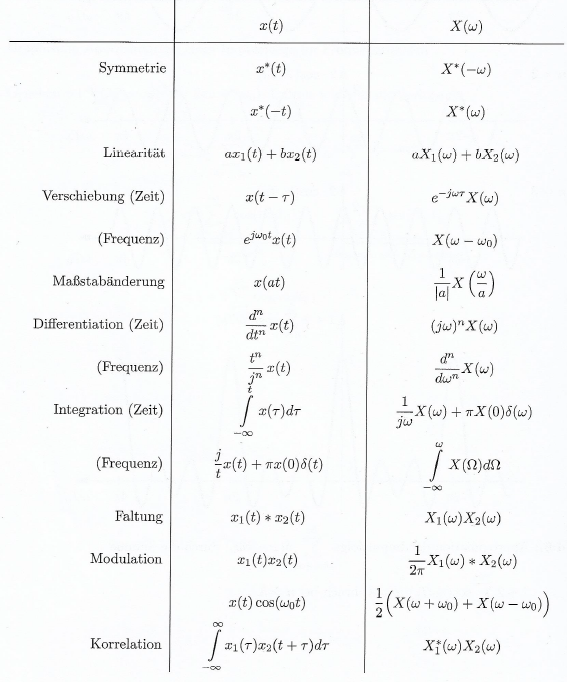
\includegraphics[scale=1]{1FourierContProperties.PNG}
\caption{A list of properties of the Fourier transformation}
\label{FourierContProperties}
\end{figure}
\begin{figure}[H]
\centering
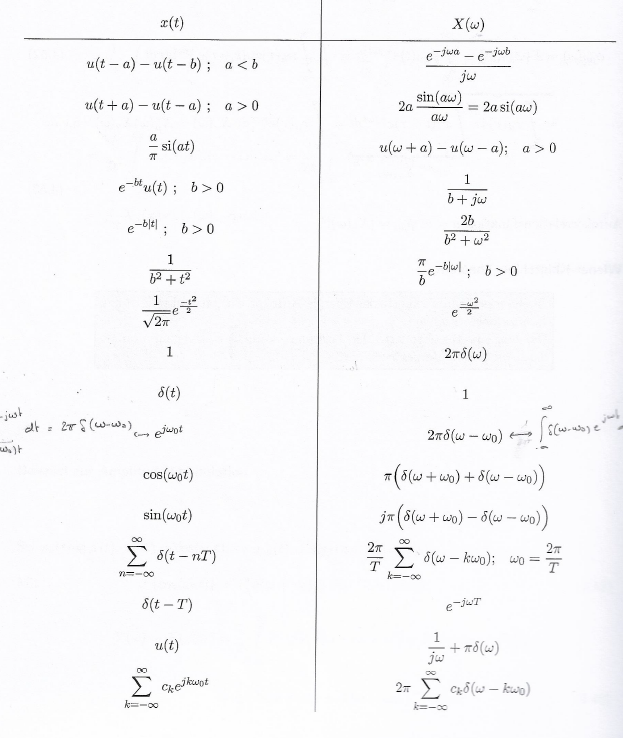
\includegraphics[scale=1]{1FourierContIdentities.PNG}
\caption{A list of known Fourier transformations}
\end{figure}

\newpage
\subsection{Time Discrete Fourier transformation}
$$
X(\Omega) = \sum_{n=-\infty}^{\infty} x[n] e^{-j \Omega n} \qquad
x[n] = \frac{1}{2\pi} \int_{2\pi} X(\Omega)e^{j \Omega n} d\Omega
$$
\begin{figure}[H]
\centering
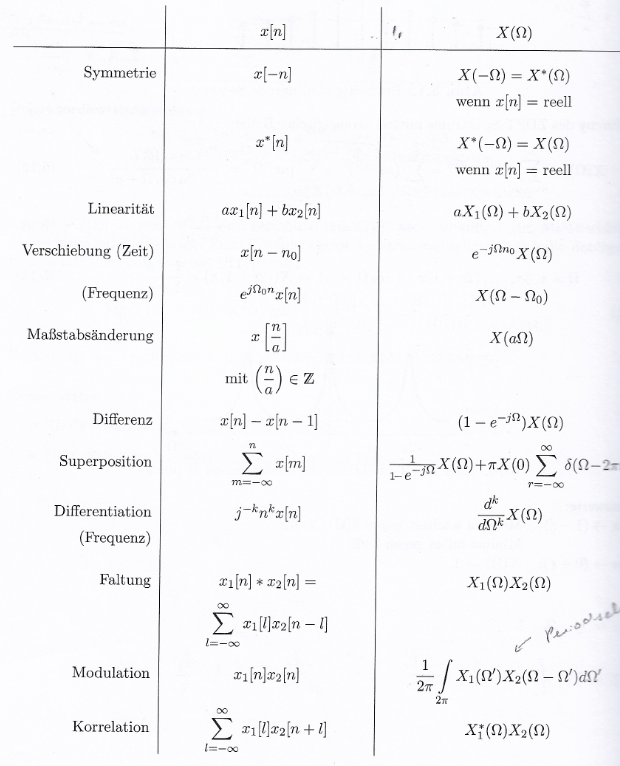
\includegraphics[scale=1]{2FourierDiscreteProperties.PNG}
\caption{A list of properties of the Time Discrete Fourier transformation}
\label{FourierContProperties}
\end{figure}
\begin{figure}[H]
\centering
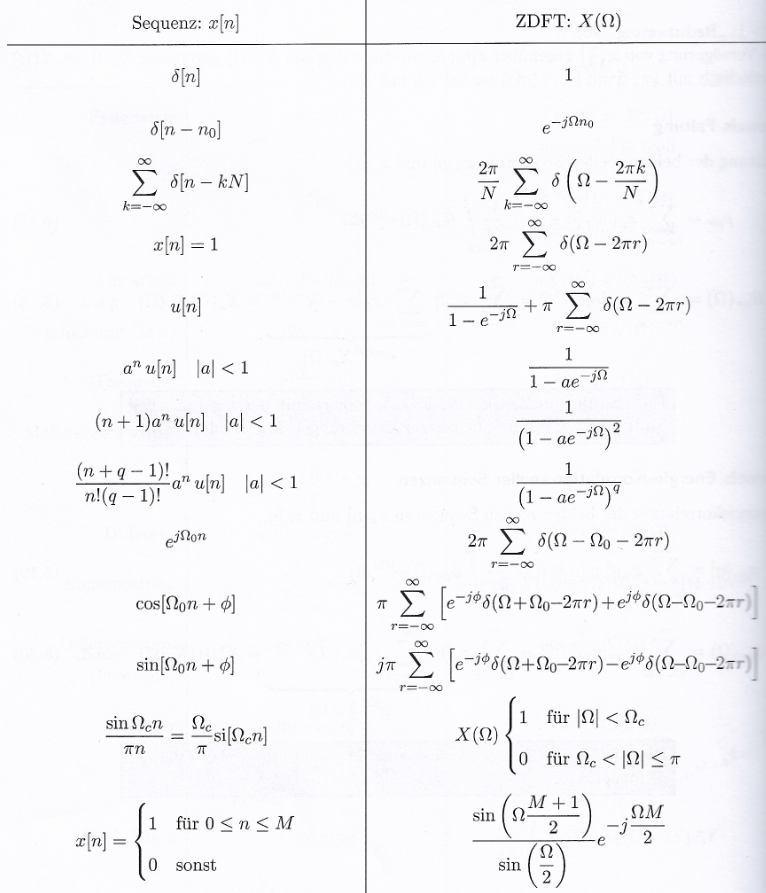
\includegraphics[scale=0.9]{2FourierDiscreteIdentities.PNG}
\caption{A list of known Time Discrete Fourier transformations}
\end{figure}

\newpage
\subsection{Laplace transformation}
$$
X(s) = \int_{-\infty}^{\infty} x(t)e^{-st}dt \qquad
x(t) = \frac{1}{2\pi j} \int_{\sigma-\infty}^{\sigma+\infty} X(s)e^{st}ds
$$
\begin{figure}[H]
\centering
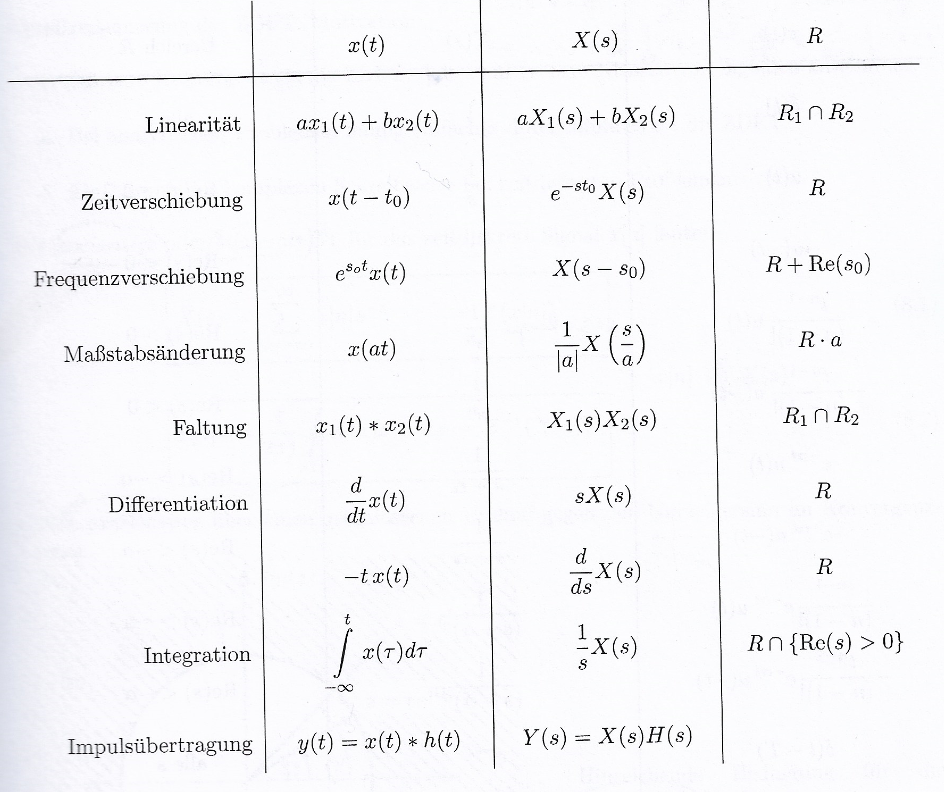
\includegraphics[scale=0.8]{3LaplaceProperties.PNG}
\caption{A list of properties of the Laplace transformation}
\label{FourierContProperties}
\end{figure}
\begin{figure}[H]
\centering
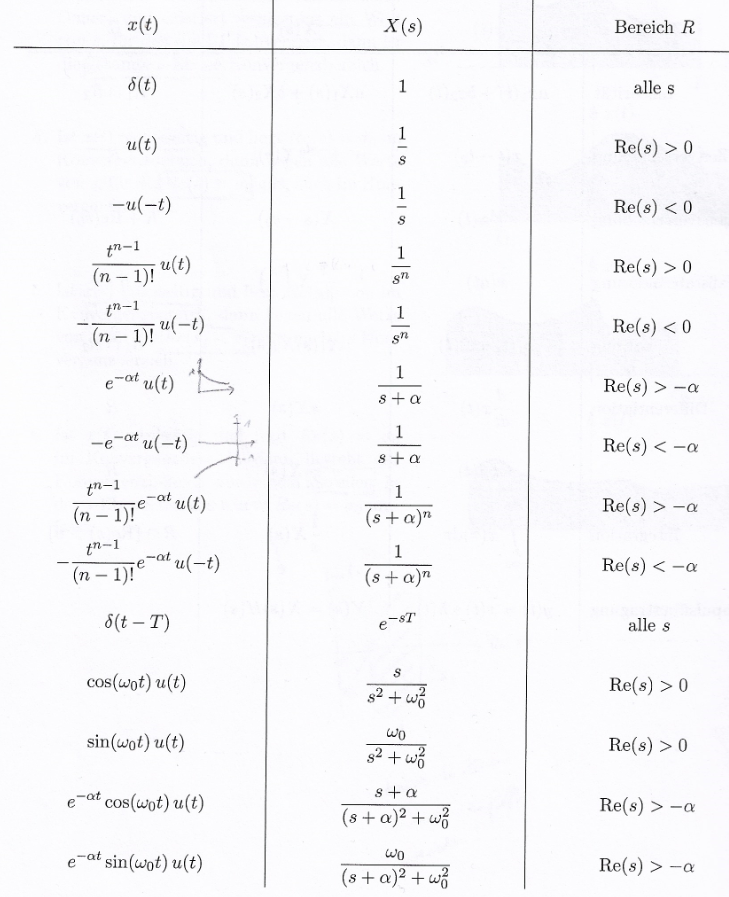
\includegraphics[scale=0.9]{3LaplaceIdentities.PNG}
\caption{A list of known Laplace transformations}
\end{figure}

\newpage
\subsection{Z-transformation}
$$
X(z) = \sum_{n=-\infty}^{\infty} x[n] z^{-n} \qquad
x[n] = \frac{1}{2\pi j} \oint_C X(z)z^{n-1} dz
$$
\begin{figure}[H]
\centering
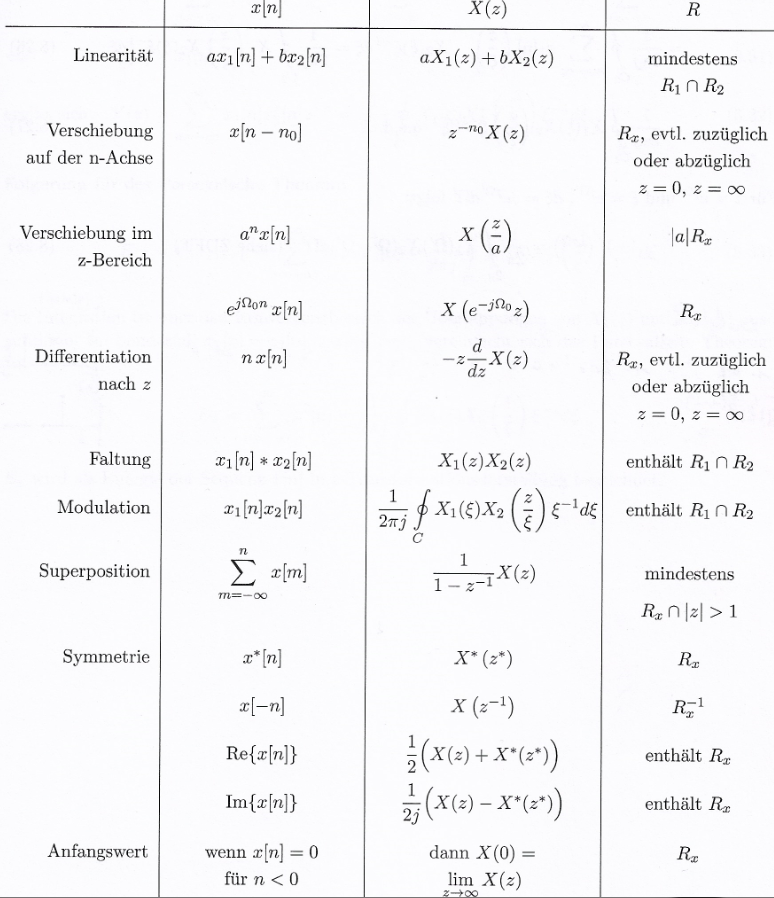
\includegraphics[scale=0.9]{4ZProperties.PNG}
\caption{A list of properties of the z-transformation}
\label{FourierContProperties}
\end{figure}
\begin{figure}[H]
\centering
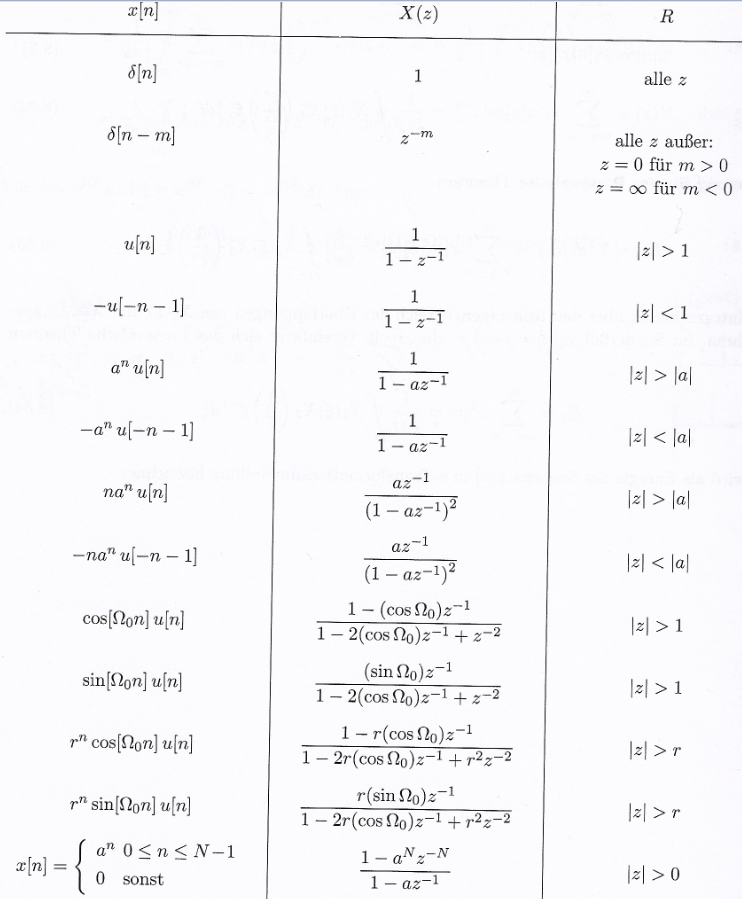
\includegraphics[scale=0.9]{4ZIdentities.PNG}
\caption{A list of known z-transformations}
\end{figure}

\section{Complement}
\subsection{Solving Differential Equations}
\begin{sidewaysfigure}
\begin{figure}[H]
\centering
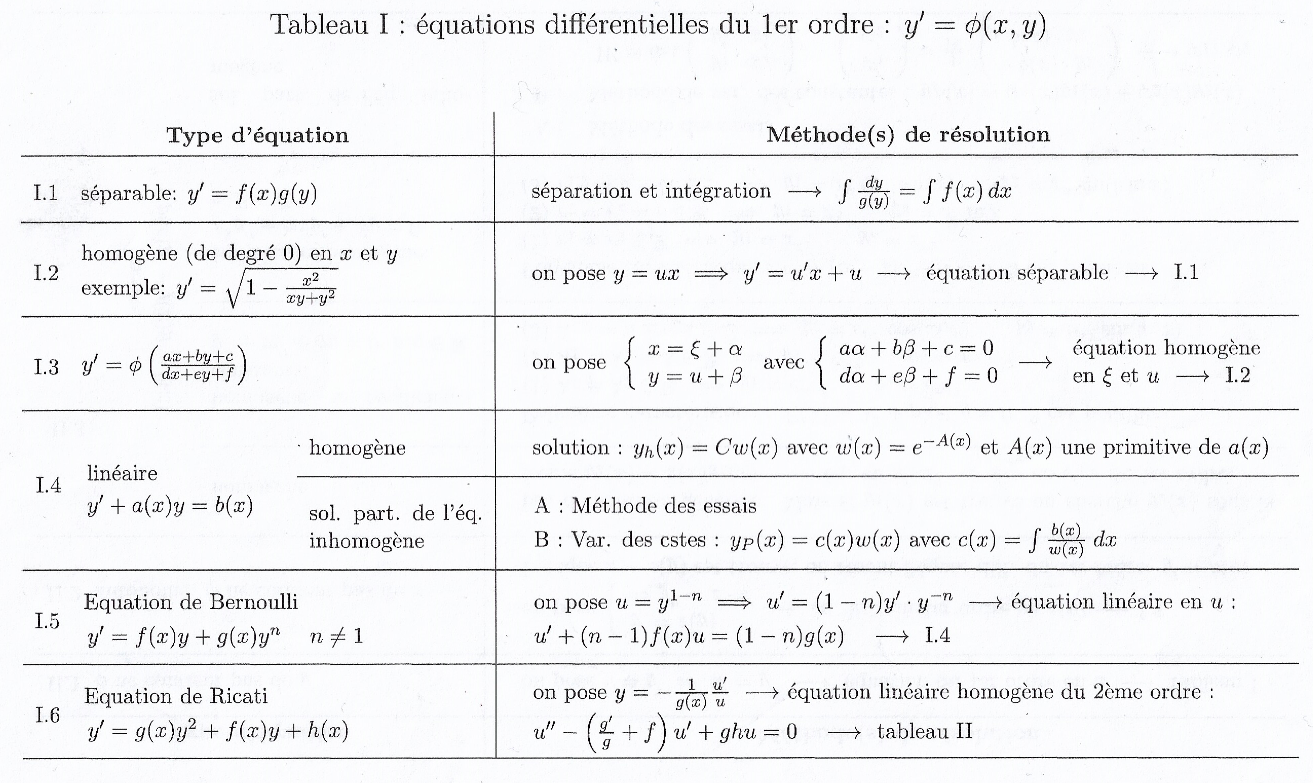
\includegraphics[scale=0.7]{EquaDiff_1.PNG}
\caption{Methods for solving first order differential equations.}
\end{figure}
\end{sidewaysfigure}

\begin{sidewaysfigure}
\begin{figure}[H]
\centering
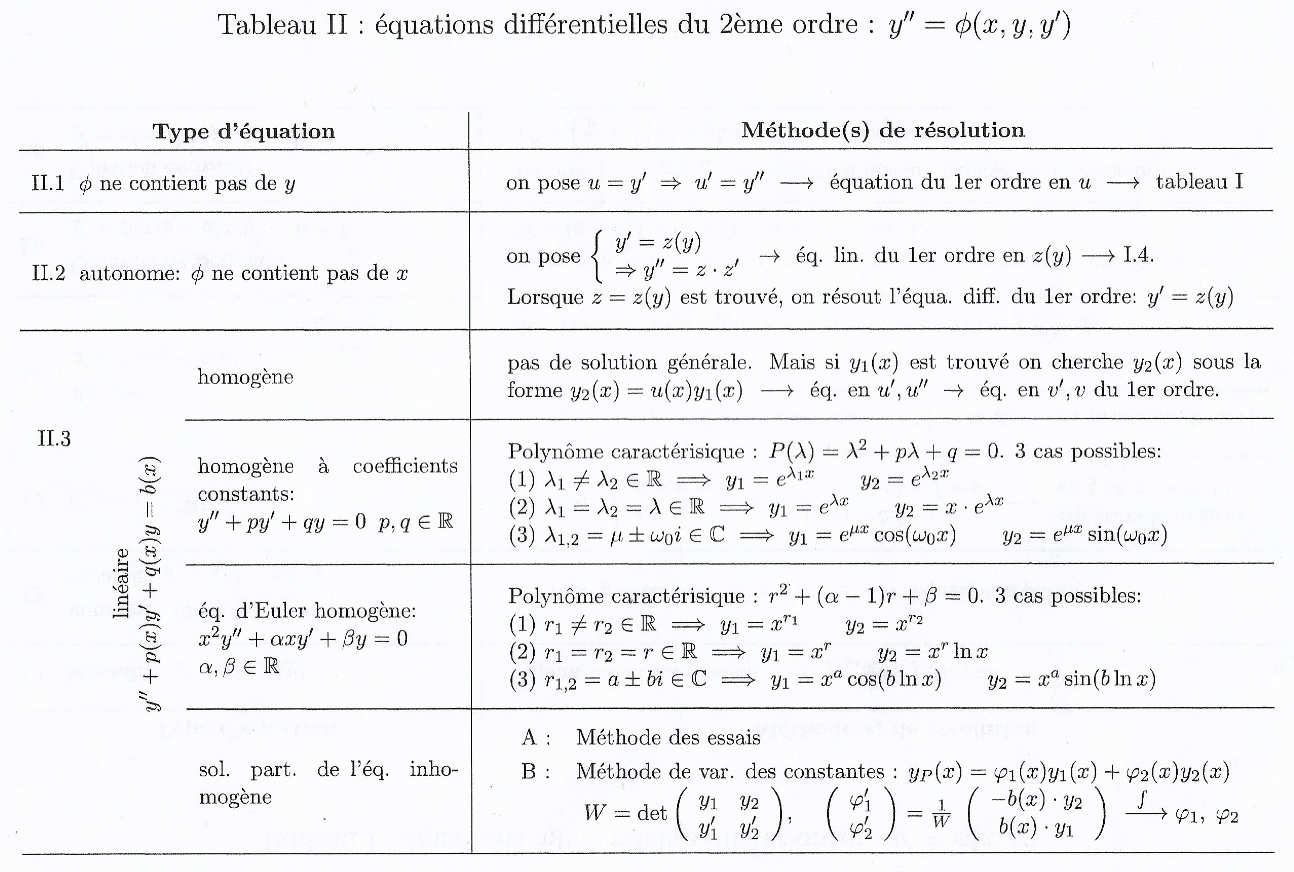
\includegraphics[scale=0.7]{EquaDiff_2.PNG}1
\caption{Methods for solving second order differential equations.}
\end{figure}
\end{sidewaysfigure}

\end{document}